\section{Task 2: Tree-Code}
\begin{frame}[plain]
	\huge{Tree-Code - Multipole Expansion}
\end{frame}

\subsection{Multipole Expansion}
\begin{frame}{Hierarchical Grouping}
	\begin{columns}
		\column{.35\linewidth}
		\begin{itemize}
			\item Octree
			\item Axis-aligned cubes
			\item Every particle is a leaf node
			\item Empty cubes not stored
			\item Children have $c^\prime = \frac{1}{2}c$ side length
		\end{itemize}
		\column{.65\linewidth}
		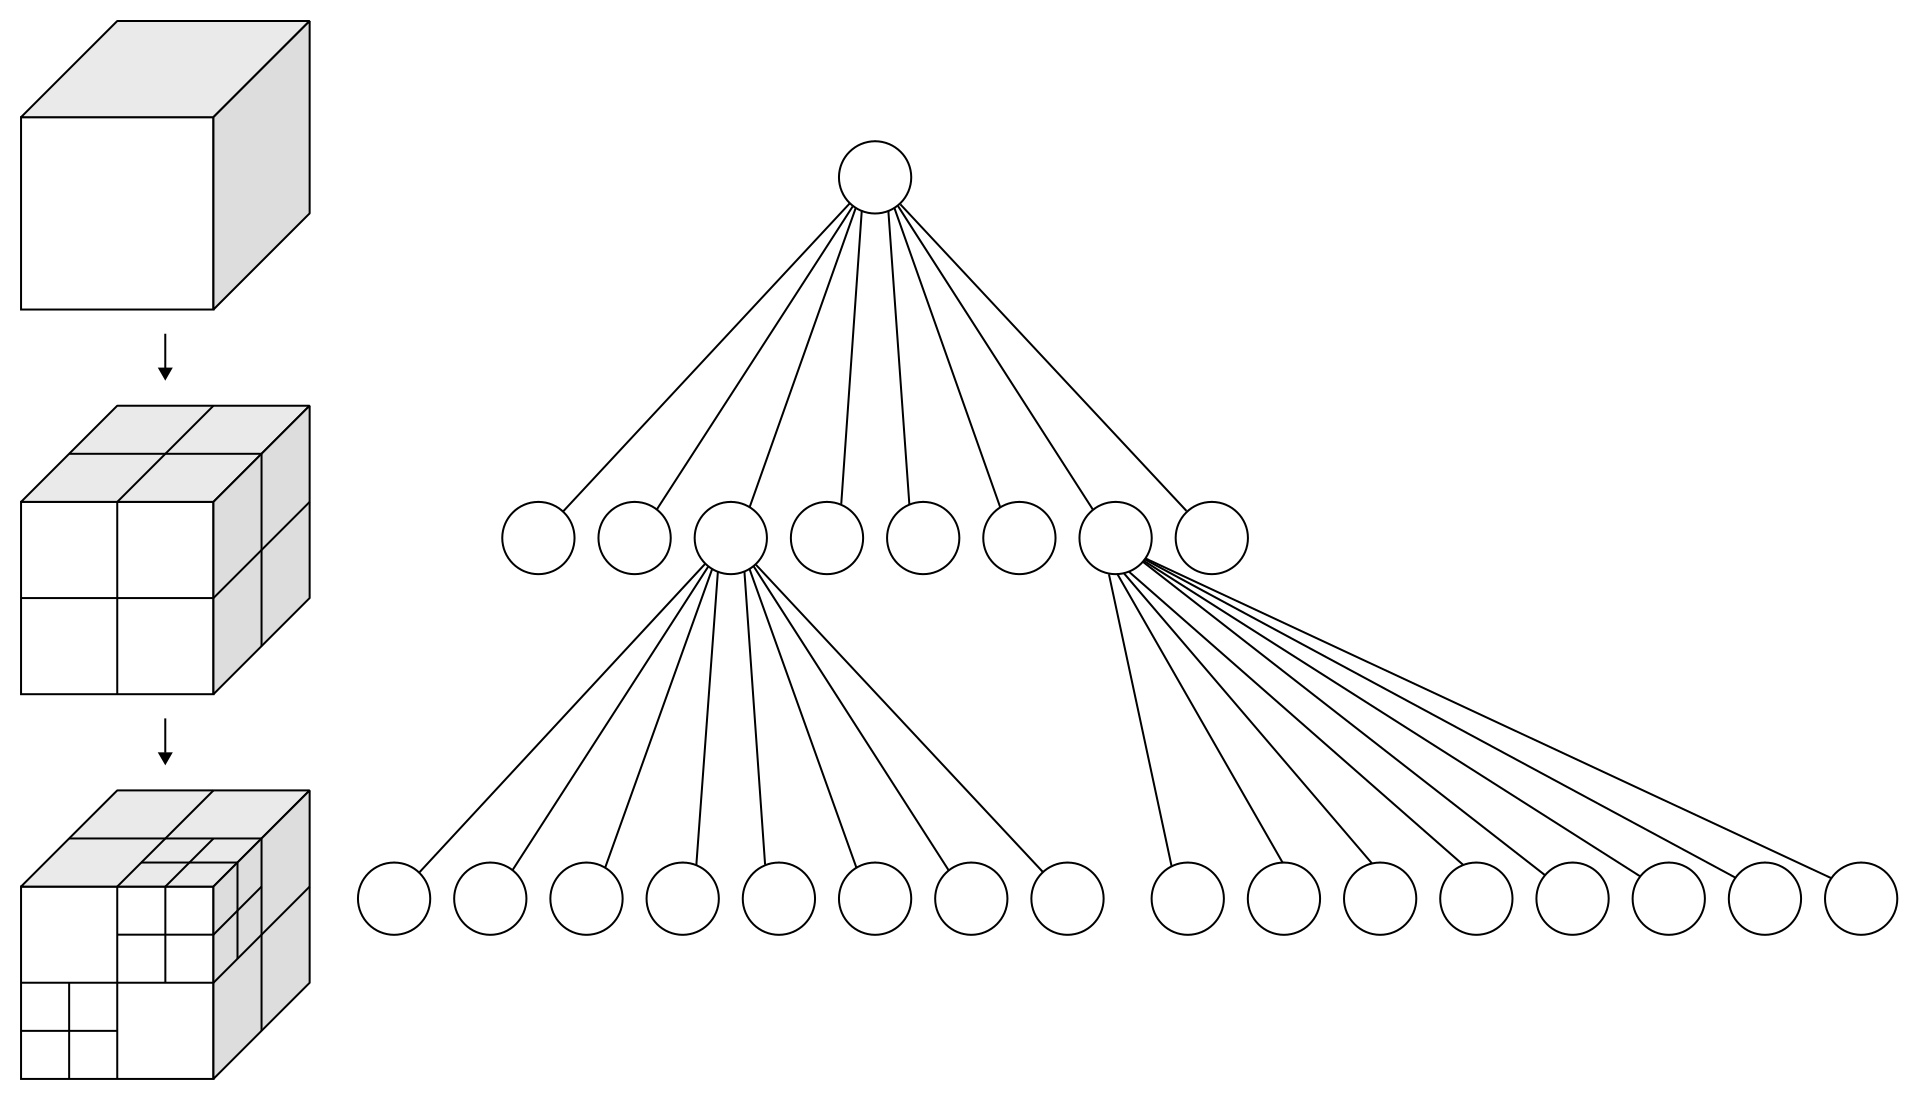
\includegraphics[width=\linewidth]{figures/cube.png}
	\end{columns}
\end{frame}

\begin{frame}[plain]{Octree}
	\includegraphics[width=\textwidth]{figures/plots/treecode.png}
\end{frame}

\begin{frame}{Multipole Expansion}
	\begin{columns}
		\column{.5\linewidth}
		\begin{itemize}
			\item $\vb{r}$ is sufficiently far
			      away
			\item  Seen under small opening angle
			      $\theta$
			\item  Orders of multipole corrections
		\end{itemize}
		\column{.5\linewidth}
		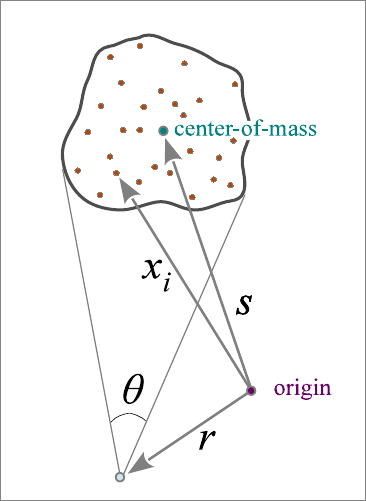
\includegraphics[width=\linewidth]{figures/multipole.png}
	\end{columns}
\end{frame}

\begin{frame}{Multipole Moments}
	\begin{itemize}
		\item Monopole
		      \begin{equation}
			      M = \sum_i m_i
		      \end{equation}
		\item Center of Mass
		      \begin{equation}
			      \vb{s} = \frac{1}{M}\sum_im_i\vb{x_i}
		      \end{equation}
		\item Quadrupole, Tensor calculation ($\vb{Q} \in \mathbb{R}^{3\times3}$)
		      \begin{equation}
			      \vb{Q}_{i j}=\sum_k m_k\left[3\left(\mathbf{s}-\mathbf{x}_k\right)_i\left(\mathbf{s}-\mathbf{x}_k\right)_j-\delta_{i j}\left(\mathbf{s}-\mathbf{x}_k\right)^2\right]
		      \end{equation}
	\end{itemize}
\end{frame}

\begin{frame}{Gravitational Potential \& Force}
	\begin{itemize}
		\item Potential:
		      \begin{equation}
			      \Phi(\mathbf{r_i})=-G\left[\frac{M}{|\mathbf{y}|}+\frac{1}{2} \frac{\mathbf{y}^T \mathbf{Q} \mathbf{y}}{|\mathbf{y}|^5}\right], \quad \mathbf{y}=\mathbf{r}_i-\mathbf{s}
		      \end{equation}
		\item Monopole Force:
		      \begin{equation}
			      \vb{F}_M(\vb{r}_i) = -G \frac{m_i  M}{ | \vb{y} | ^3}\vb{y}
		      \end{equation}
		\item Quadrupole Force:
		      \begin{equation}
			      \vb{F}_Q(\vb{r}_i) = G\left[\frac{\vb{Q}\vb{y}}{ | \vb{y} | ^4} - \frac{5}{2}
				      \frac{\vb{y}^T \vb{Q} \vb{y}} { | \vb{y} | ^4} \vb{y}\right]
		      \end{equation}
		\item Total Force:
		      \begin{equation}
			      \vb{F}(\vb{r}_i) = \vb{F}_M + \vb{F}_Q
		      \end{equation}
	\end{itemize}
\end{frame}

\begin{frame}{When to apply the expansion?}
	\begin{itemize}
		\item Opening angle:
		      \begin{equation}
			      \theta \approx \frac{c}{|\vb{y}|}
		      \end{equation}
		\item Tolerance Angle $\theta_c \in [0.5, 1]$
		\item In the limit $\theta_c \rightarrow 0$  direct summation force.
	\end{itemize}\bigskip

	{\footnotesize
		Where:
		\begin{itemize}
			\item $c$ - Length of cube side
			\item $\vb{y}$ - Vector: particle position to center of mass
		\end{itemize}
	}
\end{frame}

\begin{frame}{Tree Walk}
	\begin{itemize}
		\item Depth-First traversal
	\end{itemize}
	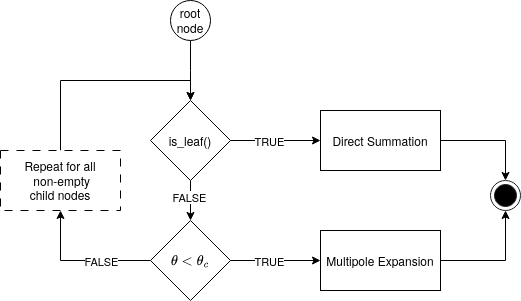
\includegraphics[width=0.95\textwidth]{figures/multipole_uml.png}
\end{frame}

\subsection{Direct Summation}
\begin{frame}{Integration with Direct Summation}
	$T = 5 \cross t_{cross}$ in dimensionless calculation with $\Delta t = \eta t_{cross}$. \bigskip

	Iteration on each particle with \texttt{OpenMP} and on each particle \textbf{Leapfrog} integration in \textit{kick-drift-kick} form:
	\begin{itemize}
		\item $v_{n+1/2} = r_0 + a_0  \frac{\Delta t}{2}$
		\item $r_{n+1} = r_0 + v_{n+1/2} \Delta t$
		\item $a_{n+1} = df(\Delta t)$
		\item $v_{n+1} = v_{n+1/2} + a_{n+1} \frac{\Delta t}{2}$
	\end{itemize} \bigskip

	{\footnotesize Where:
		\begin{itemize}
			\item $\eta = [0.1, 0.01]$
			\item $t_{cross} \approx 6e^{-6}$
			\item $df(\Delta t)$ - Direct force summation
		\end{itemize}
	}

	\bigskip\centering
	SHOW GIFS

\end{frame}

\begin{frame}{Force Comparison - Accuracy}
	Assumption: Direct Force summation considered most accurate. \\

	$\lim\limits_{\theta_c \to 0}$ leads to Direct Summation, often considered in the range of $[0.5, 1.0]$.
\end{frame}

\begin{frame}[allowframebreaks]{Force Comparison}
	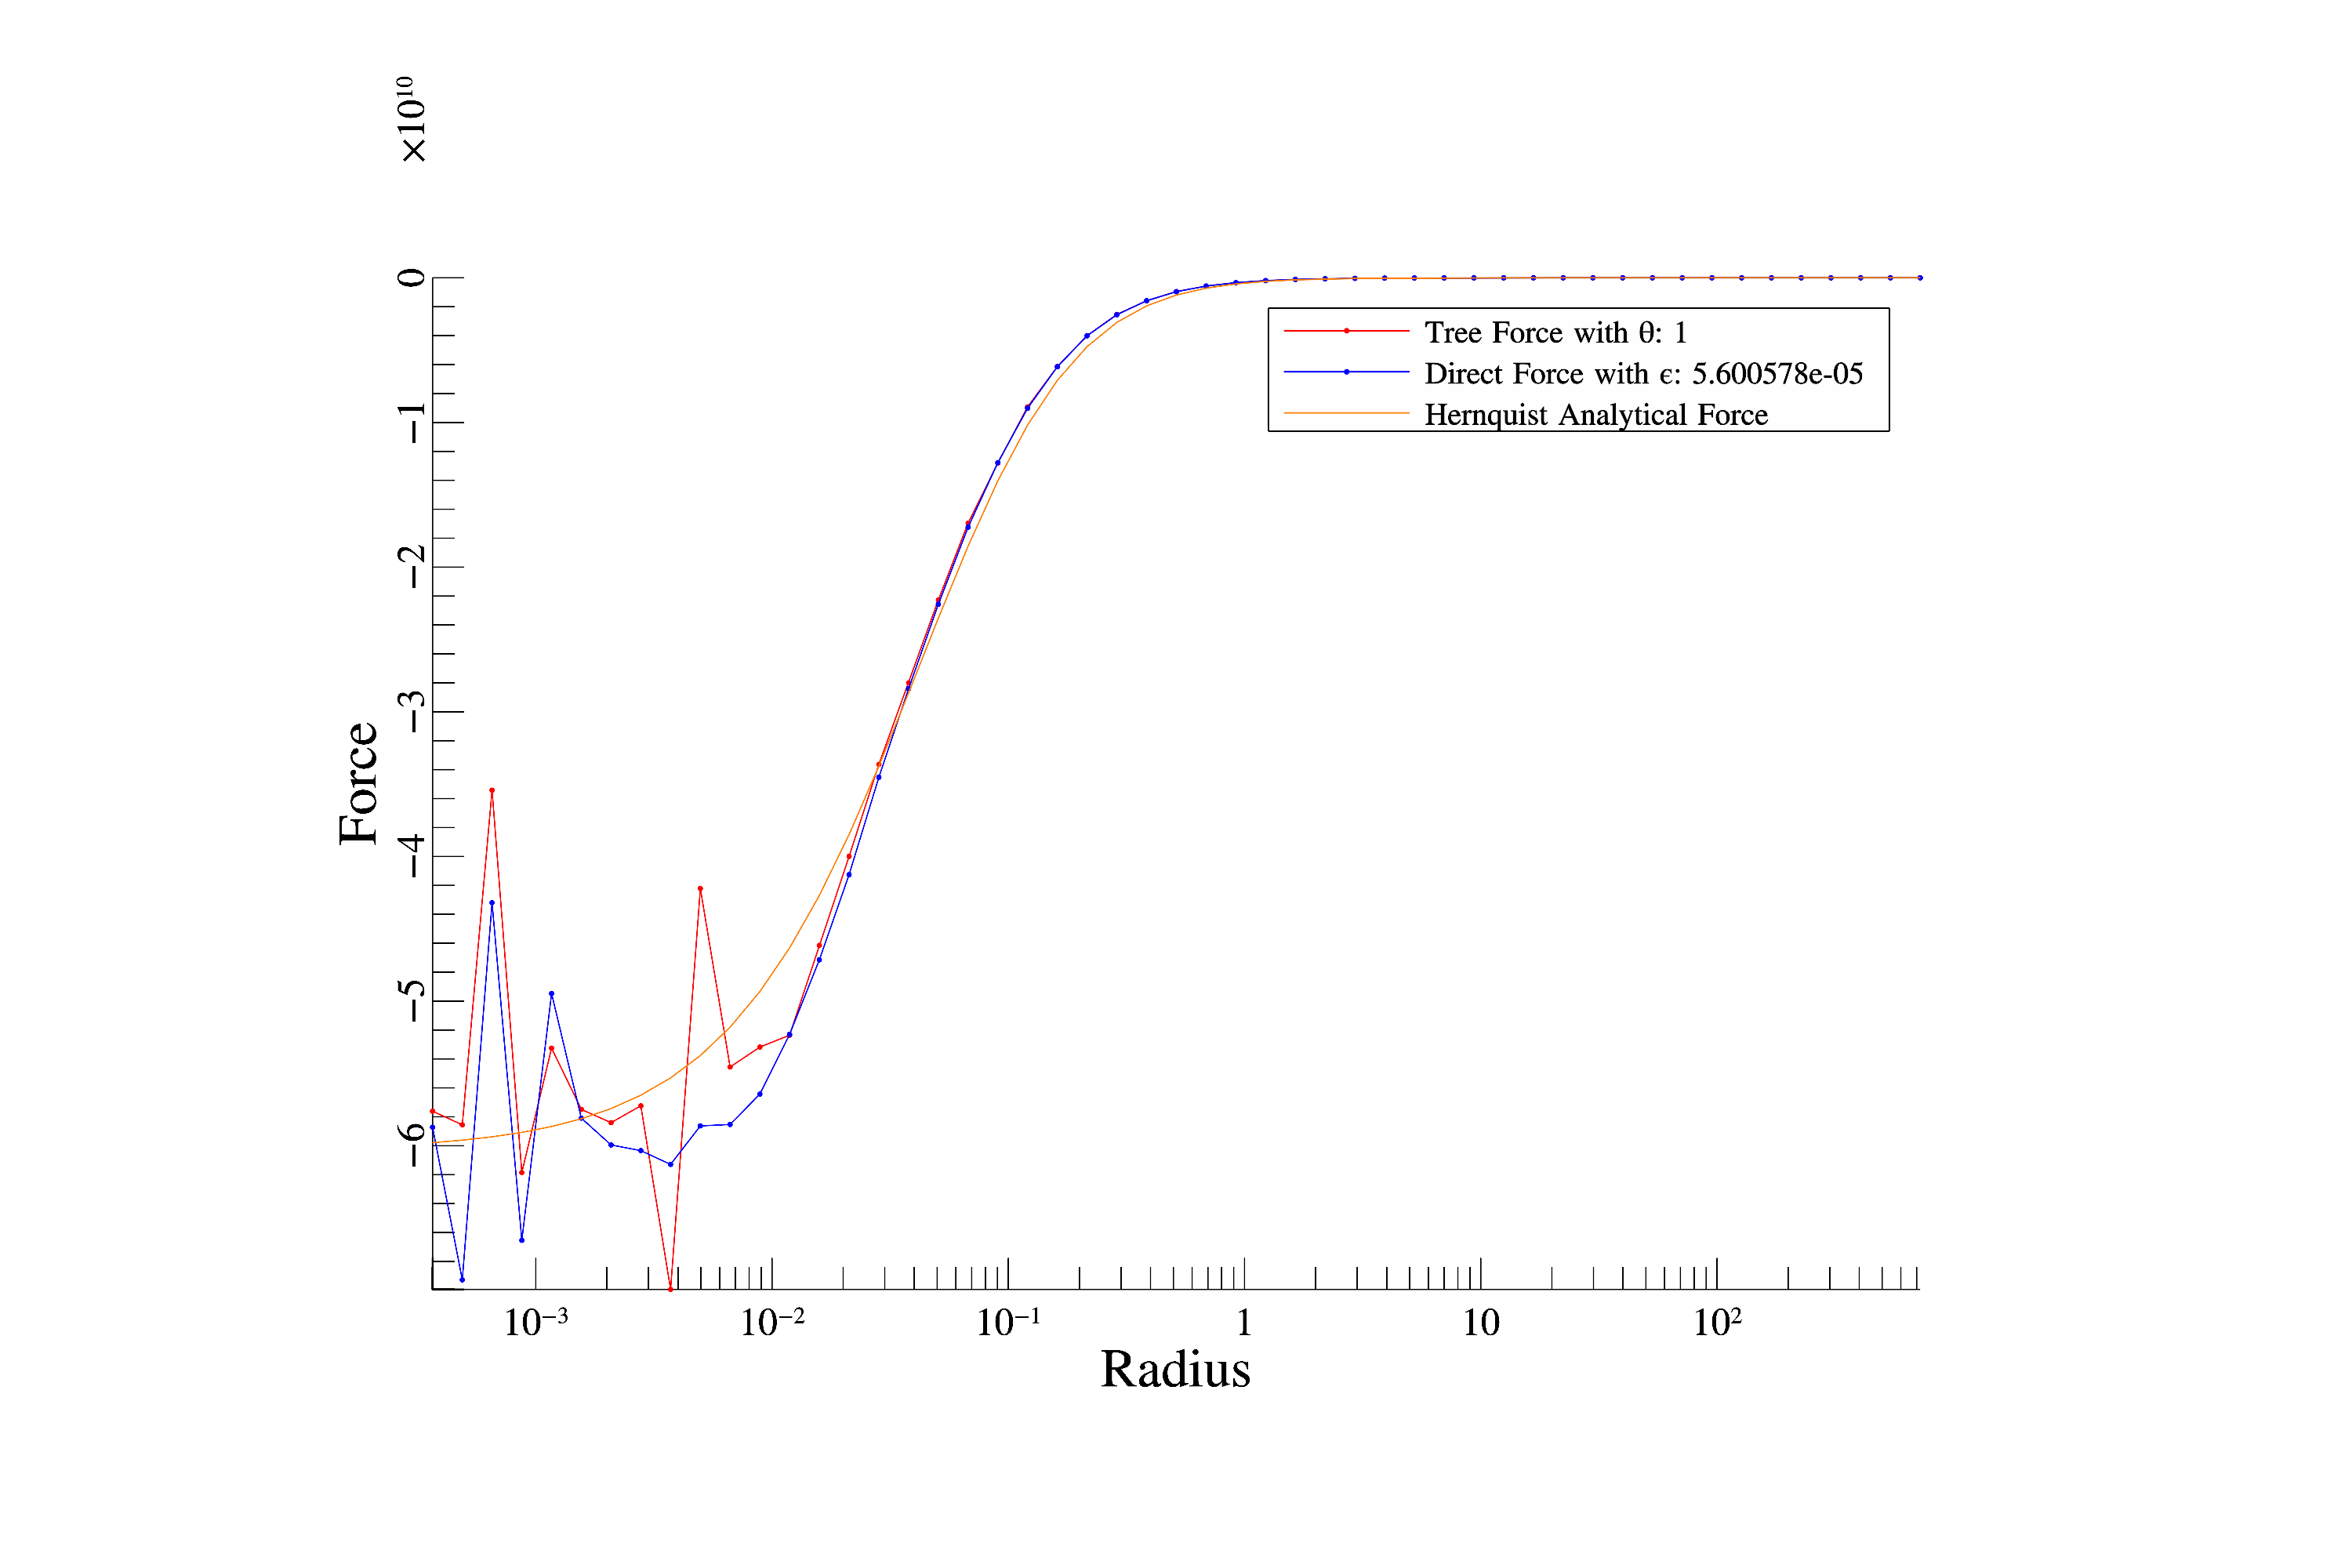
\includegraphics[width=\textwidth]{figures/plots/tree_force_1.png}
	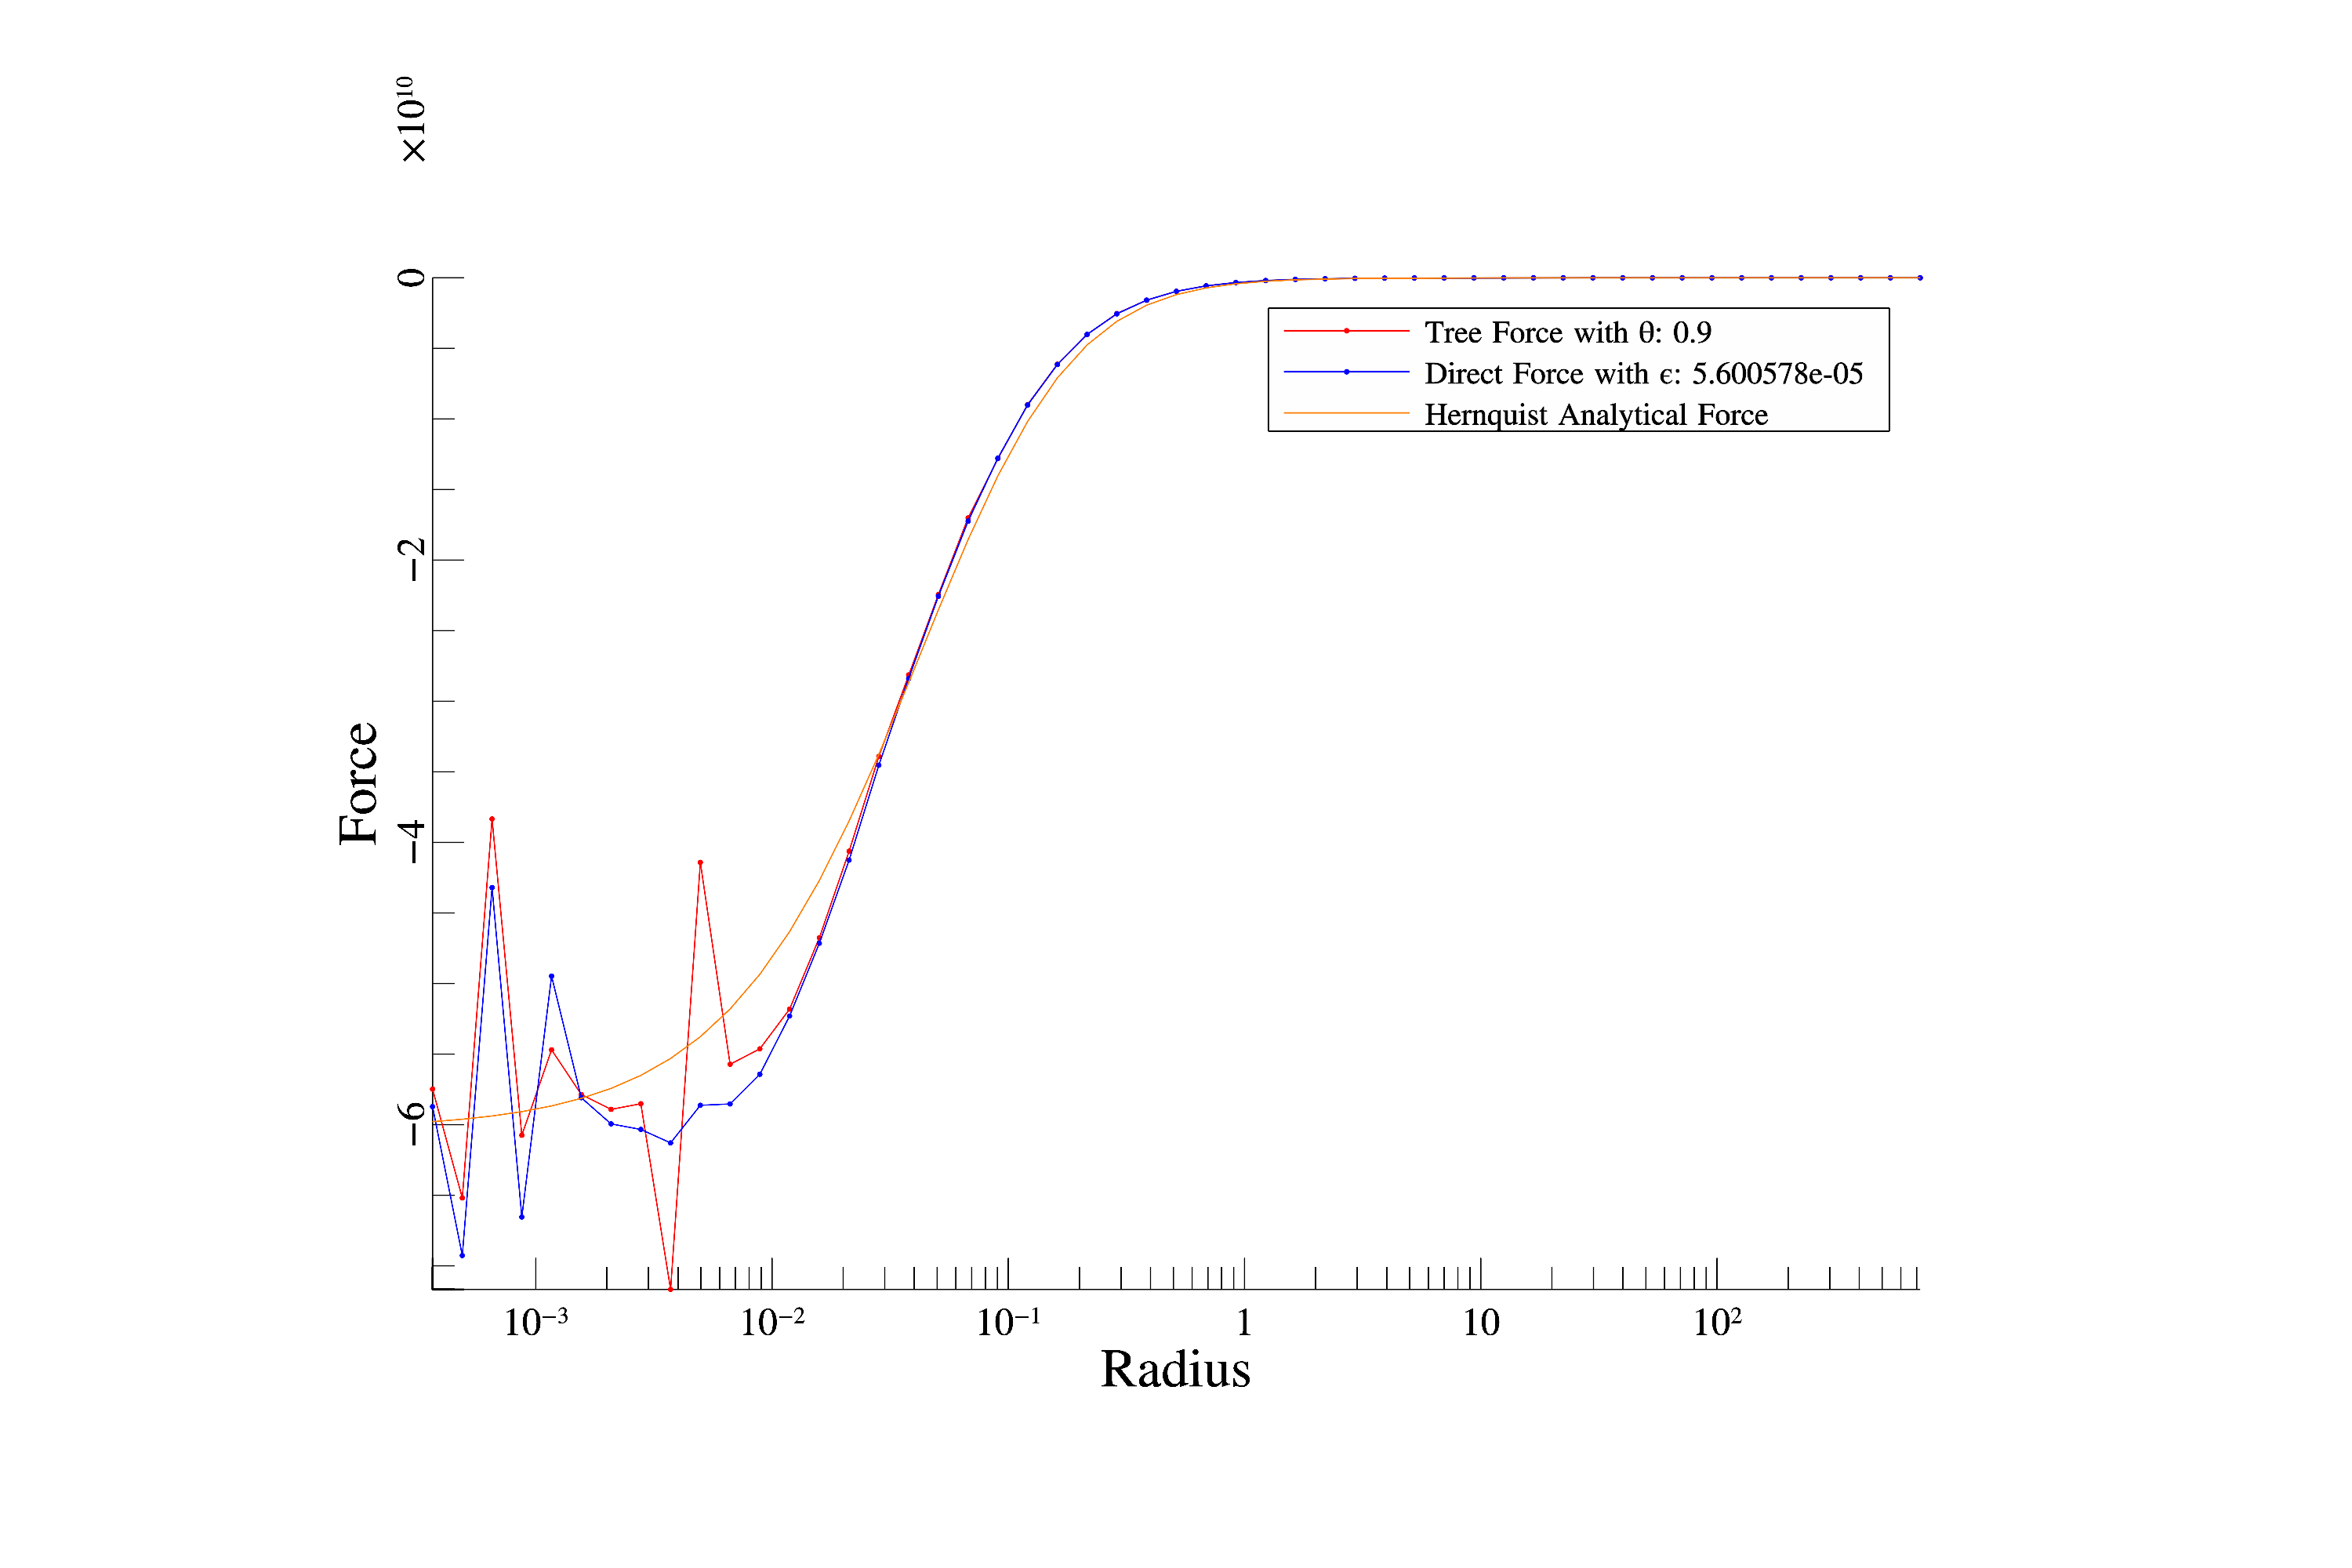
\includegraphics[width=\textwidth]{figures/plots/tree_force_0.9.png}
	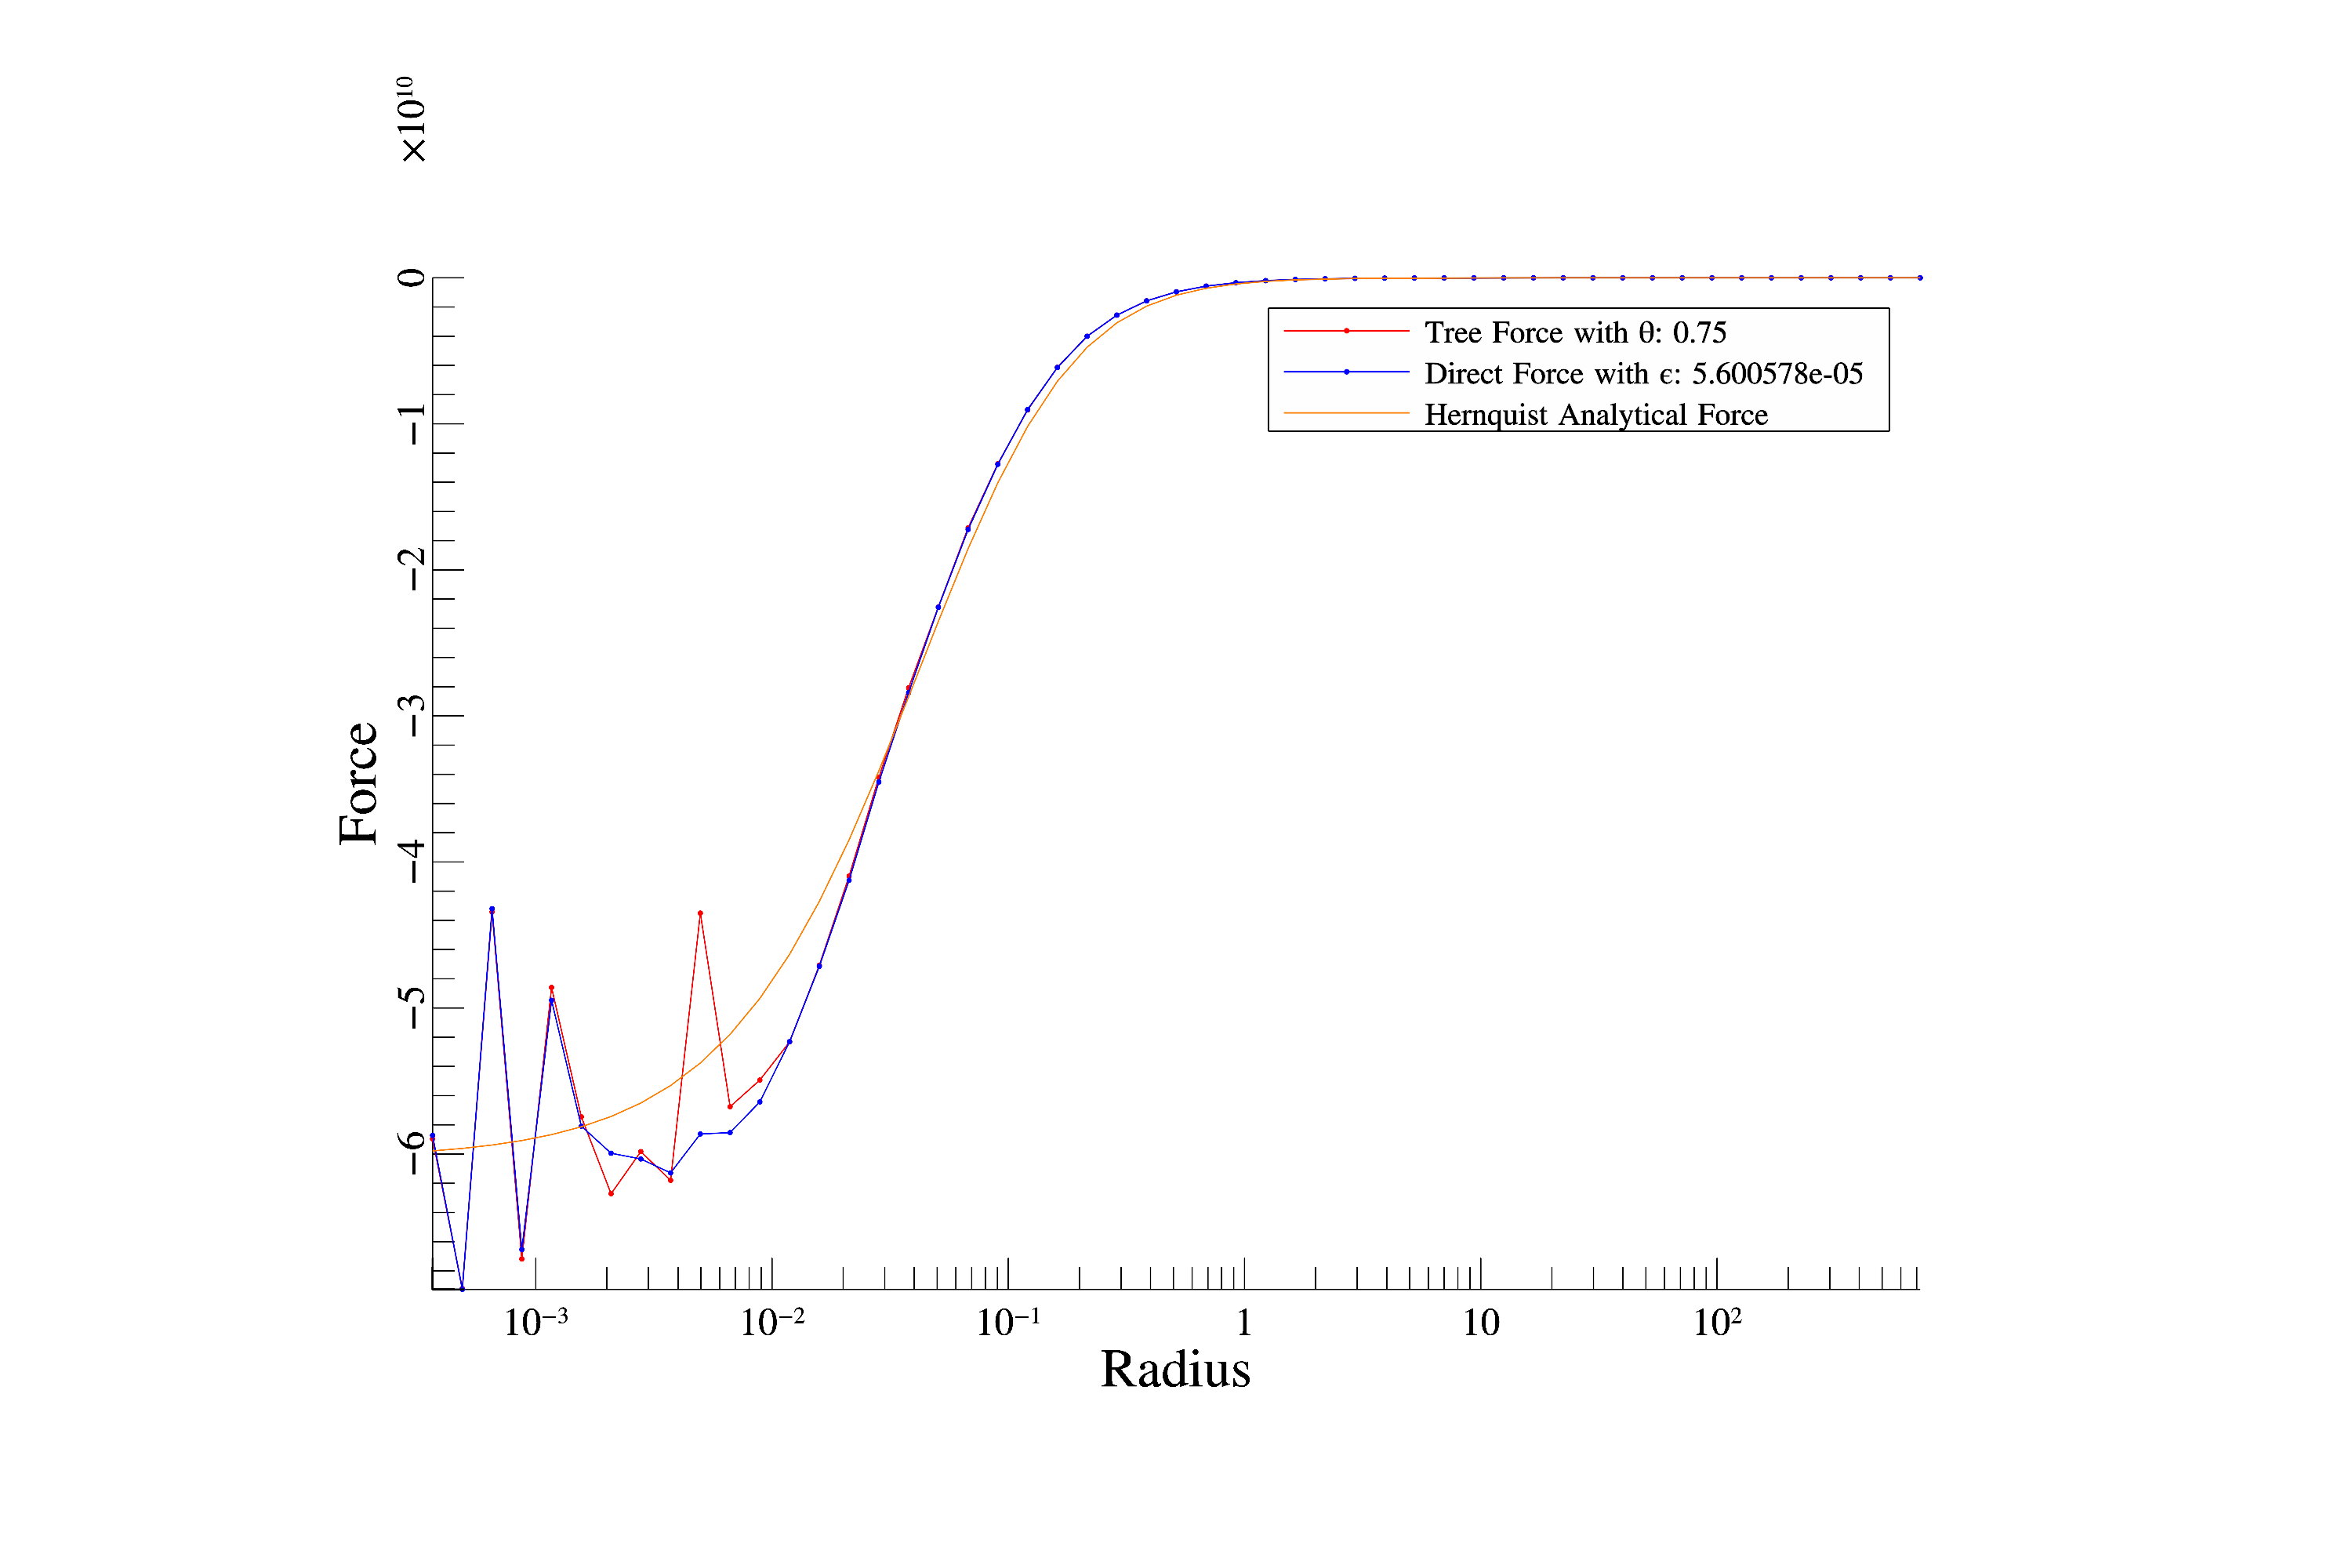
\includegraphics[width=\textwidth]{figures/plots/tree_force_0.75.png}
	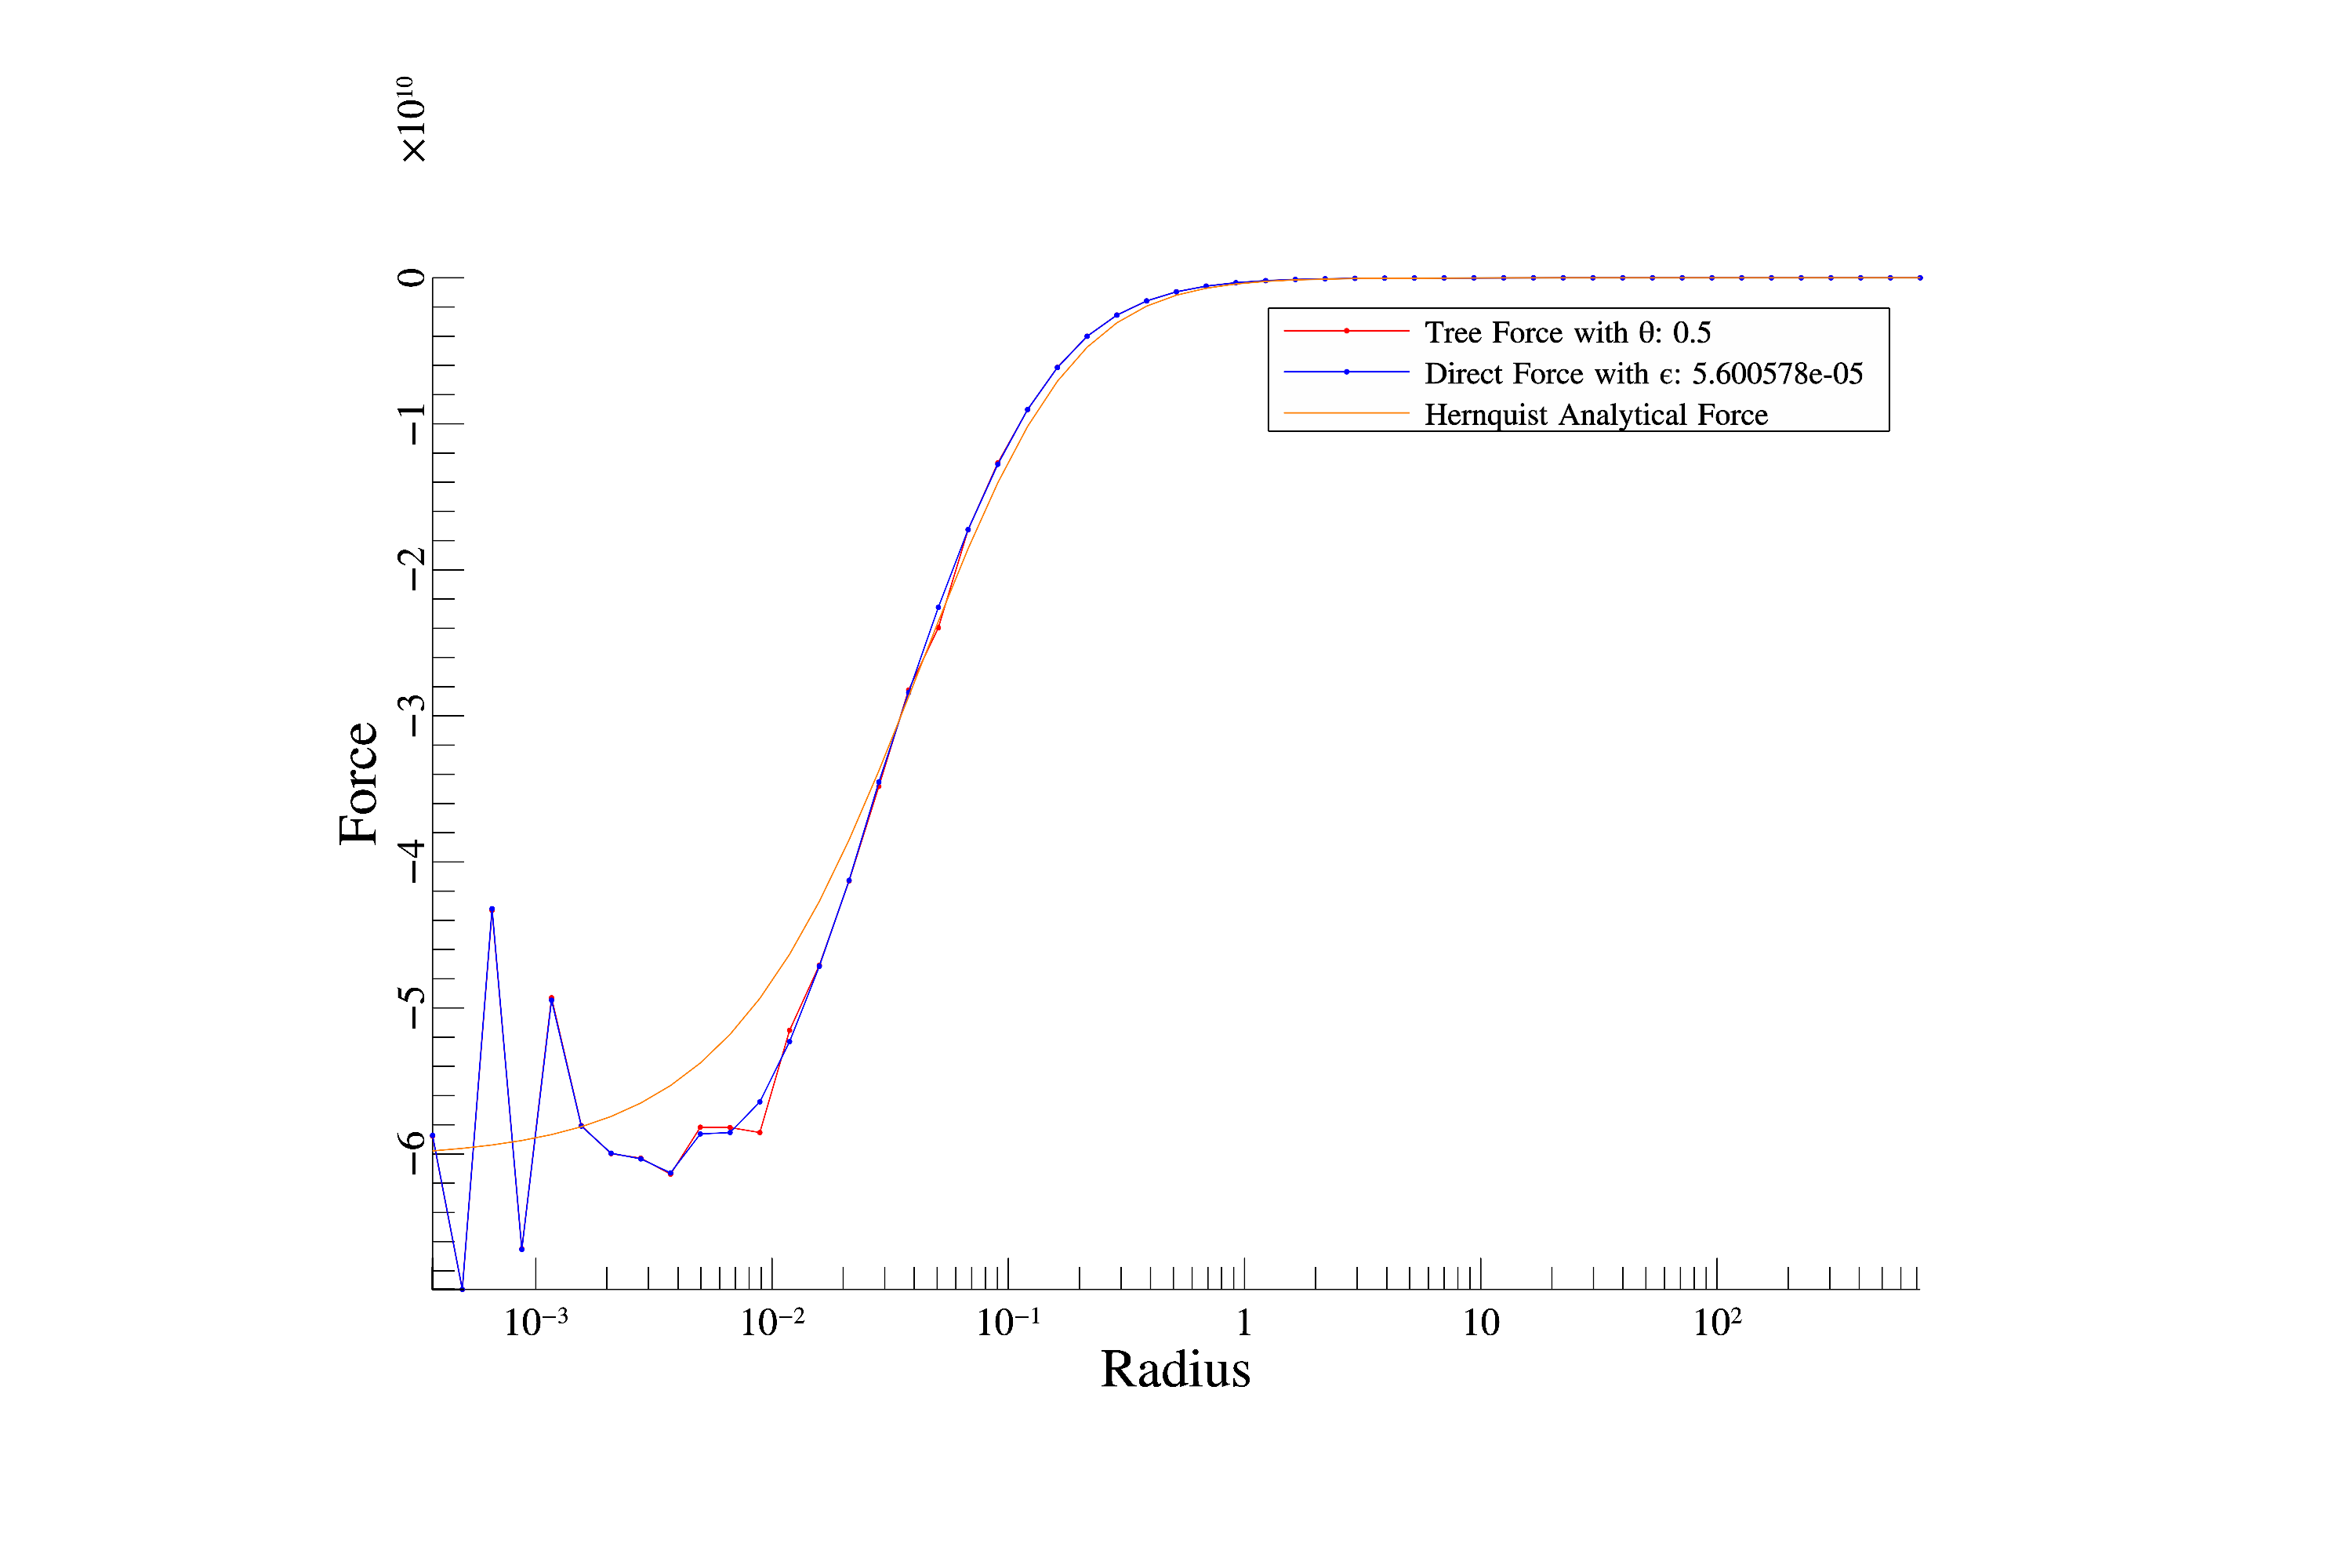
\includegraphics[width=\textwidth]{figures/plots/tree_force_0.5.png}
	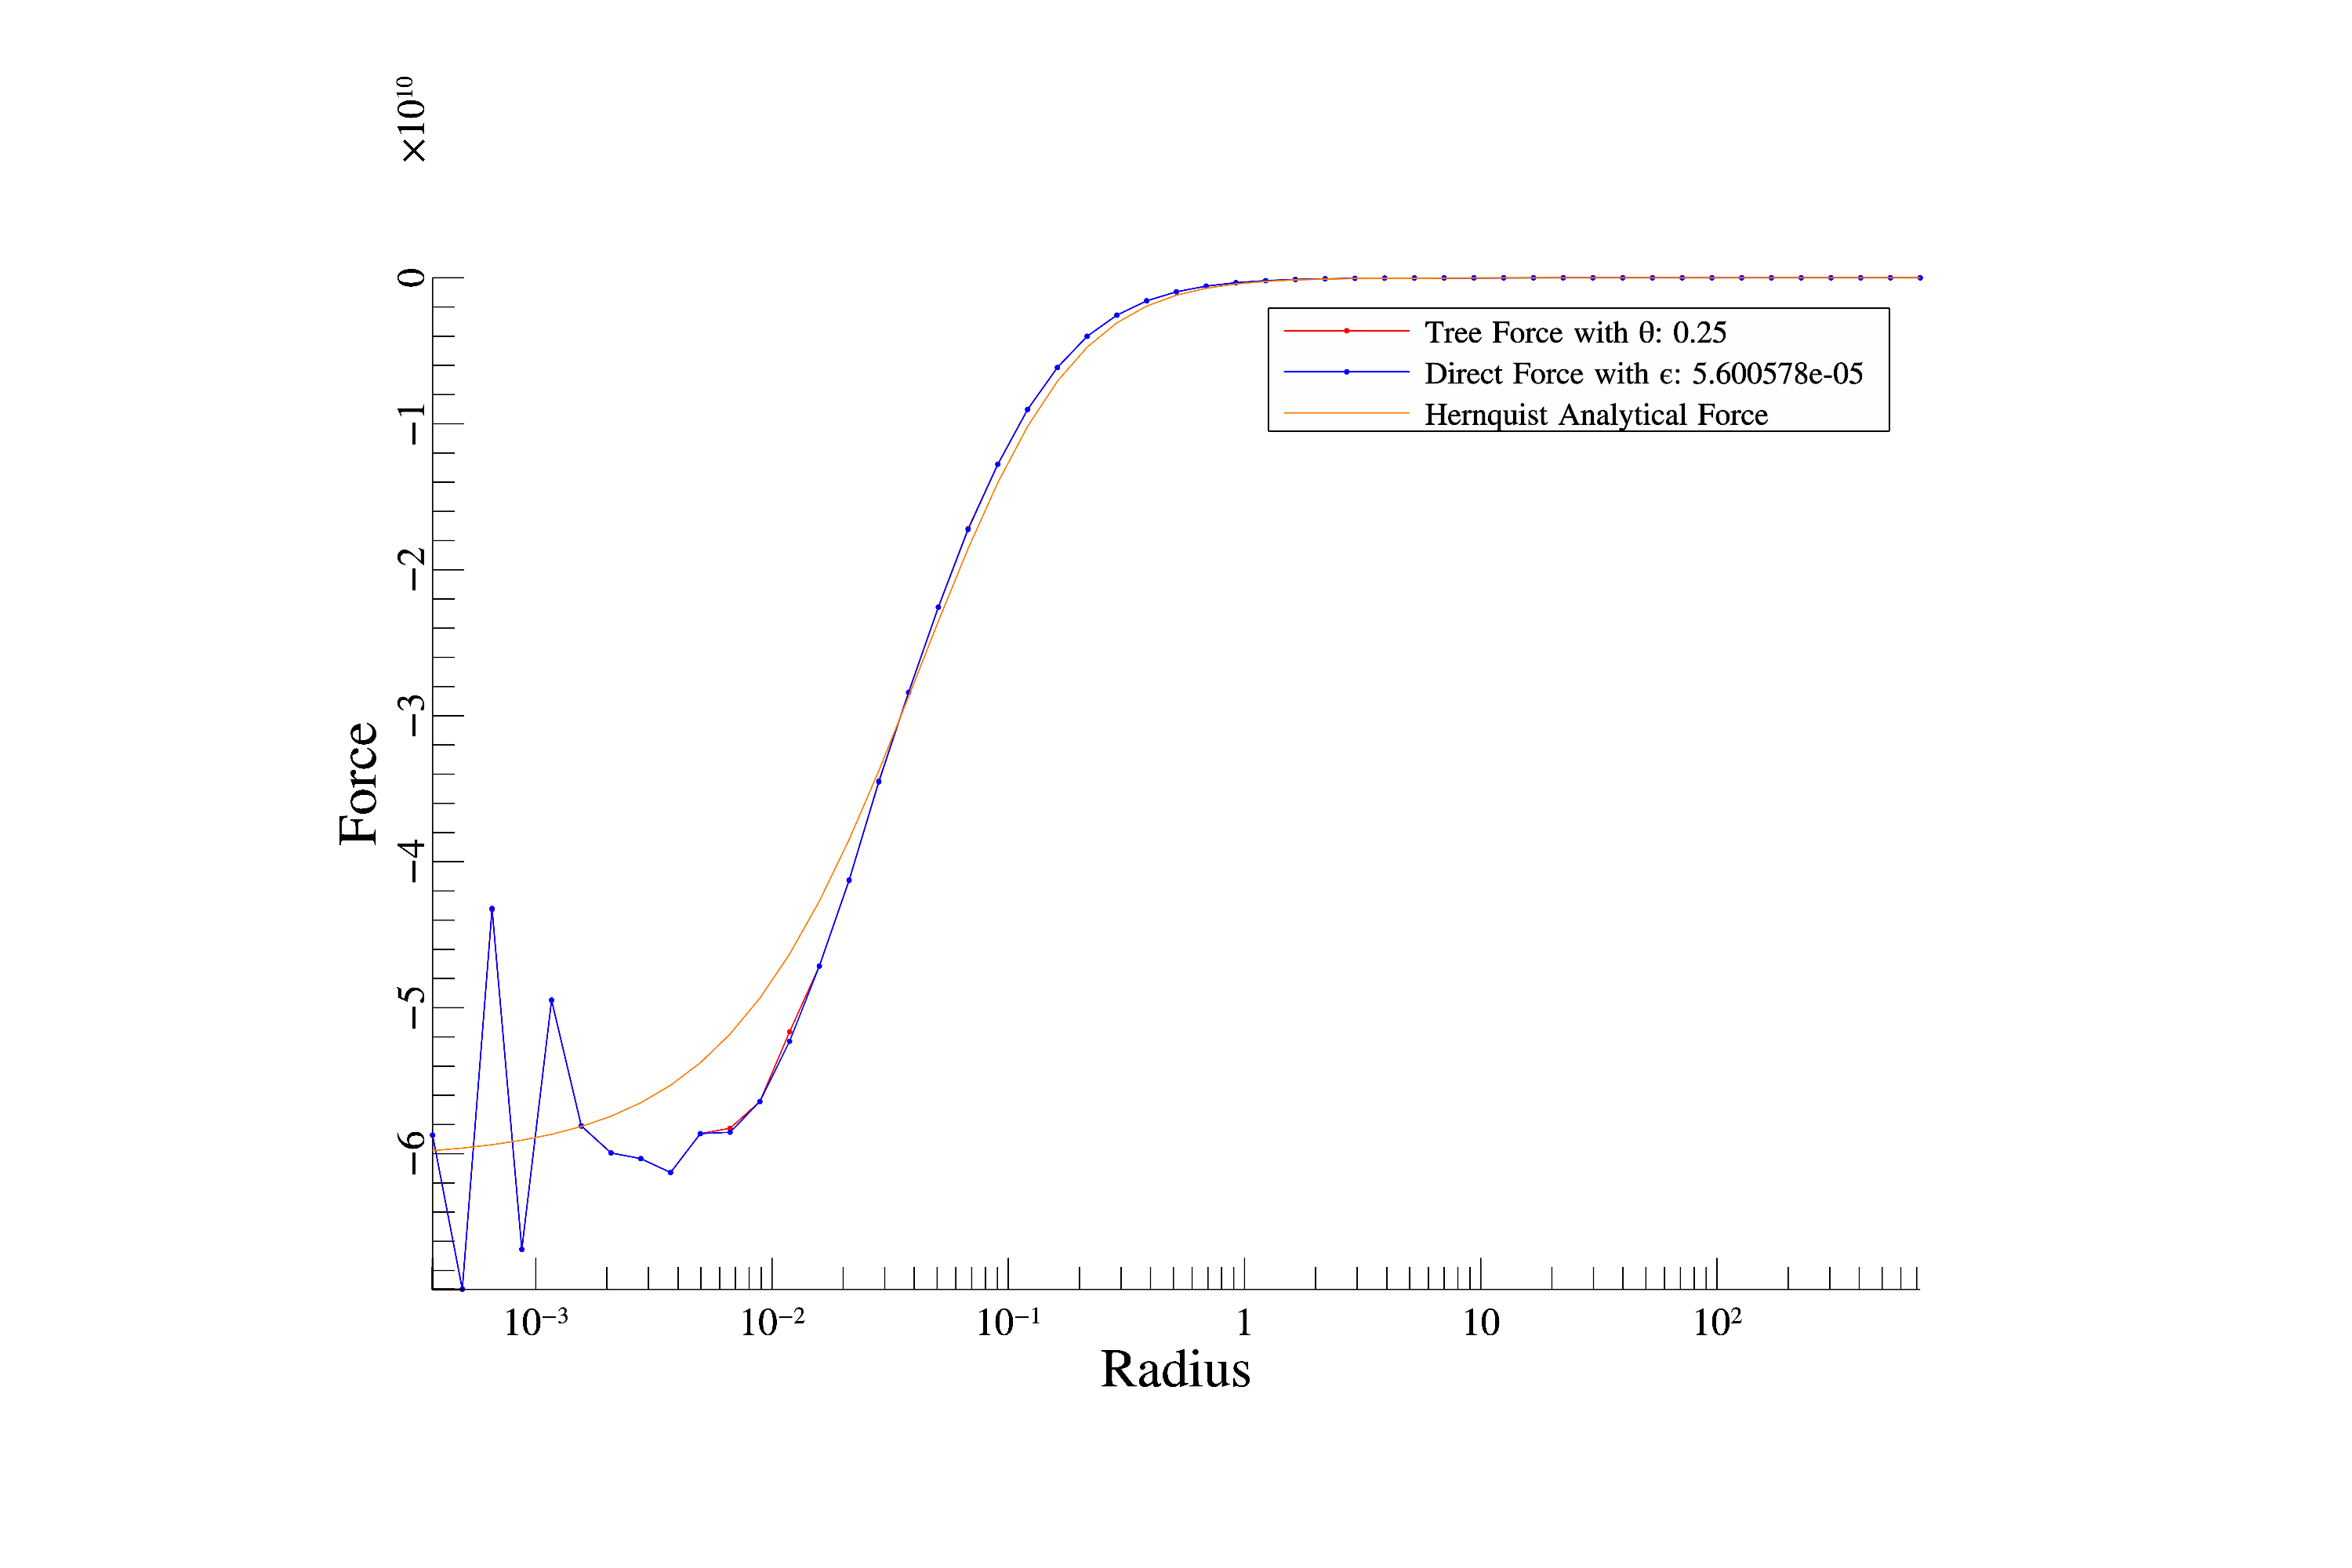
\includegraphics[width=\textwidth]{figures/plots/tree_force_0.25.png}
	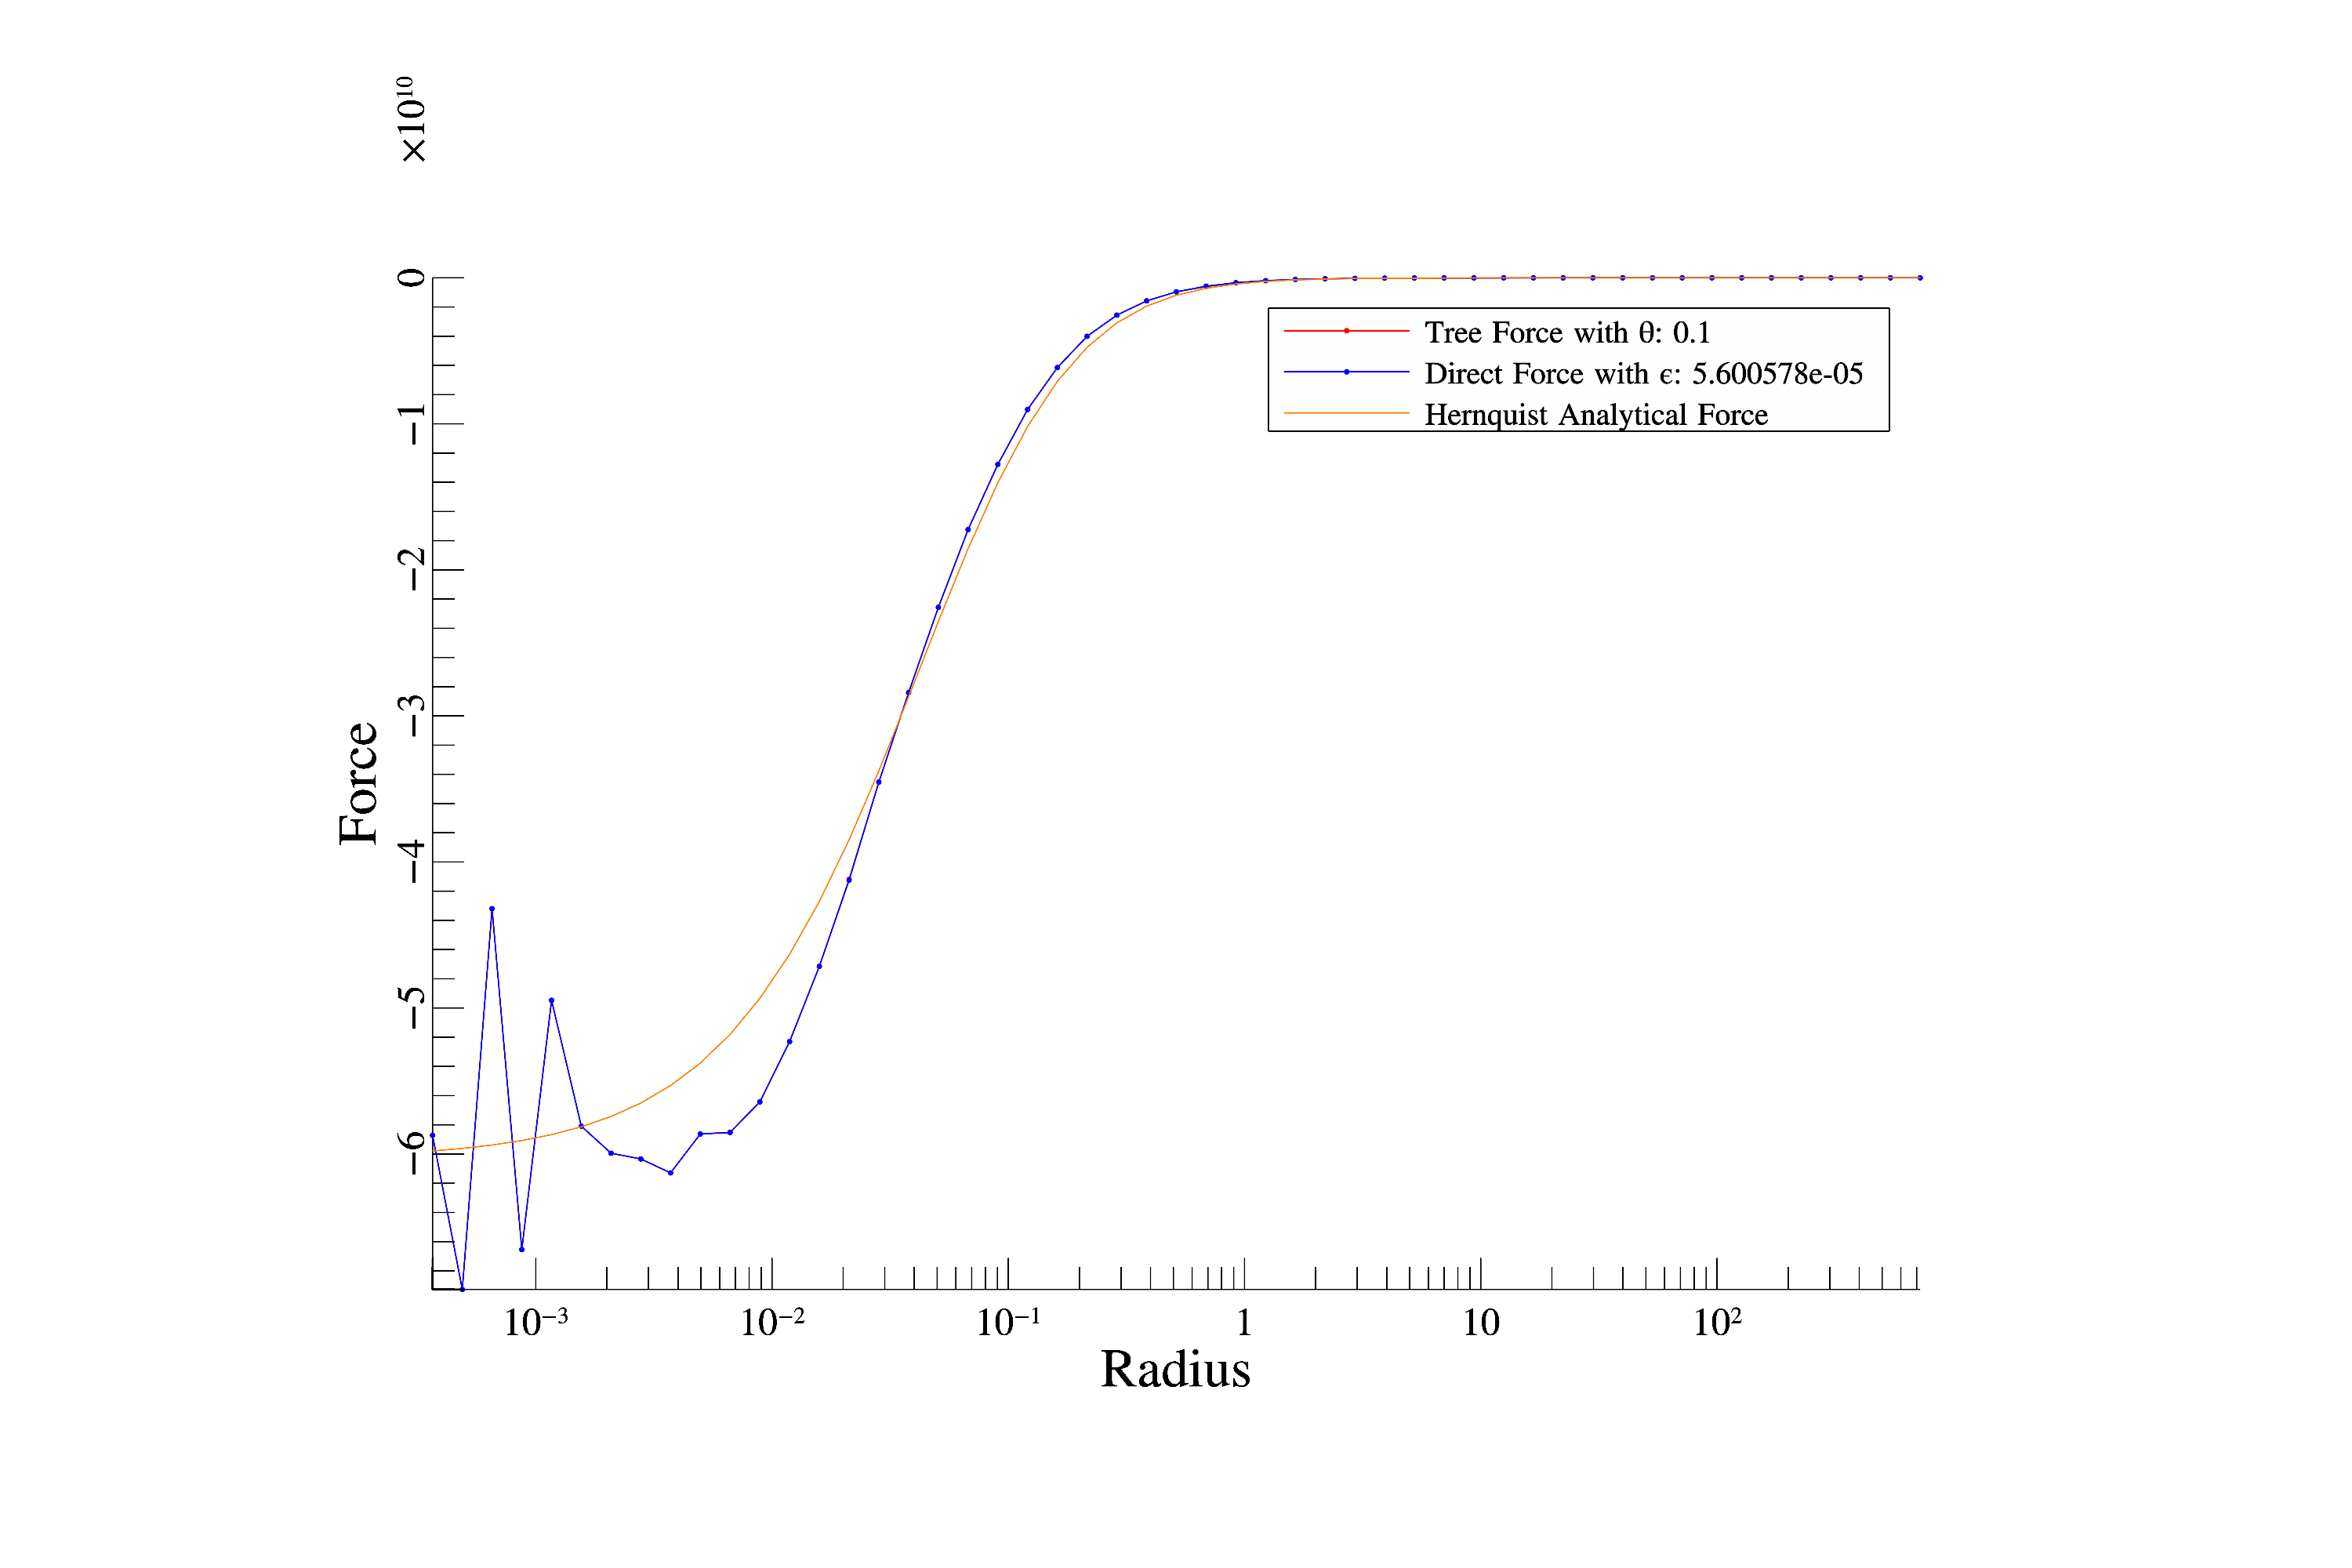
\includegraphics[width=\textwidth]{figures/plots/tree_force_0.1.png}
\end{frame}

\begin{frame}{Computational Cost Comparison}
	Direct Force Computation:
	\begin{itemize}
		\item $\mathcal{O}(N^2)$ - Comparison of each particle with every other, parallelizable
		\item $\frac{N^2}{2}$ - Comparison of each particle only with unvisited particles, not parallelizable
	\end{itemize} \bigskip


	Tree Force Computation:
	\begin{equation}
		% number of nodes needed for calculating the force on a central particle in the middle of the sphere
		N_{nodes}=\frac{4 \pi}{\theta_c^3} \ln \frac{R}{d} \propto \frac{\ln N}{\theta_c^3} .
	\end{equation}
	Expected $\mathcal{O}(N\log{N})$ but in practice values near $\approx\frac{N^2}{10'000}$
\end{frame}
